\documentclass[letterpaper,11pt]{article}
\usepackage{latexsym}
\usepackage[empty]{fullpage}
\usepackage[usenames,dvipsnames]{color}
\usepackage{verbatim}
\usepackage{hyperref}
\usepackage{framed}
\usepackage{tocloft}
\usepackage{bibentry}
\usepackage{amsmath}
\usepackage{scrextend}
\usepackage{listings}
\usepackage{color}
\usepackage{fancyhdr}
\usepackage{graphicx}

%THIS PORTION IS FOR ADDING PAGE NUMBER
\pagestyle{fancy}
\cfoot{}
\rfoot{\thepage}
\renewcommand{\headrulewidth}{0pt}
%THIS PORTION IS FOR ADDING PAGE NUMBER

\urlstyle{same}
\definecolor{mygrey}{gray}{.85}
\definecolor{mygreylink}{gray}{.30}
\textheight=9.0in
\raggedbottom
\raggedright
\setlength{\tabcolsep}{0in}


%The following part is for inserting codes in LaTeX:
\definecolor{codegreen}{rgb}{0,0.6,0}
\definecolor{codegray}{rgb}{0.5,0.5,0.5}
\definecolor{codepurple}{rgb}{0.58,0,0.82}
\definecolor{backcolour}{rgb}{0.95,0.95,0.92}

\lstdefinestyle{mystyle}{
    backgroundcolor=\color{backcolour},
    commentstyle=\color{codegreen},
    keywordstyle=\color{magenta},
    numberstyle=\tiny\color{codegray},
    stringstyle=\color{codepurple},
    basicstyle=\footnotesize,
    breakatwhitespace=false,
    breaklines=true,
    captionpos=b,
    keepspaces=true,
    numbers=left,
    numbersep=5pt,
    showspaces=false,
    showstringspaces=false,
    showtabs=false,
    tabsize=2
}
\lstset{style=mystyle}
%For inserting codes in LaTeX

\begin{document}

\begin{center}
	\textbf{\Huge{Advanced Data Analysis HW4}}
\end{center}

\begin{center}
	\textsl{Ao Liu, al3472}
\end{center}

\bigbreak
\bigbreak
\bigbreak


%%%%%%%%%%%%%%%%%%%%%%%%%%%%%%%%%%%%%
%%%%%%%%%%%%%%   1   %%%%%%%%%%%%%%%%
%%%%%%%%%%%%%%%%%%%%%%%%%%%%%%%%%%%%%


\begin{addmargin}[-2em]{0em} \large{\textbf{1. }}\end{addmargin}
\textbf{Consider the 3 player game shown below, in which player3’s strategy set is ${M1,M2,M3,M4}$. Each cell only lists one payoff, which represents all three players’ payoffs from that strategy profile. E.g., all three players’ payoff is 8 from $(A, C, M_1)$.}
\bigbreak

\textbf{Let $p \in [0, 1]$ denote the probability of playing $A$ in a mixed strategy for player 1 (so $1 - p$ is the probability of playing B), and $q \in [0, 1]$ denote that of playing $C$ in a mixed strategy for player 2 (so $1 - q$ is the probability of playing D). We can denote a mixed strategy profile for players 1 and 2 by a pair $(p, q)$.}

\begin{addmargin}[-1.1em]{0em} \textbf{(a)}\par\end{addmargin}
  \textbf{Compute the expected payoff for player 3 when she plays some $M_j$ given any mixed strategy profile for the opponents, i.e., give algebraic expressions for $v_3(M_j,p,q)$ for each $j \in {1,2,3,4}$.}\par
\bigbreak
\begin{addmargin}[-0.5em]{0em}
\textbf{Answer: }\end{addmargin}


I expect there's a positive correlation between sales of cigarettes and Age, because the people with higher ages tend to smoke more cigarettes, the proportion of people smoking within young people is relatively small.\par
I expect there's a negative correlation between sales of cigarettes and HS, because people with higher education are more aware of the harm of smoking and are tend to somke less.\par
I expect there's a positive correlation between sales of cigarettes and Income, because with more money, people can afford more cigarettes.\par
I don't expect there's a correlation between sales of cigarettes and Black, because there's no supporting evidence that black people are mode likely to smoke more than others.\par
I expect there's a negative correlation between sales of cigarettes and Female, because there are a lot more men smoking than women, the higher the proportion of the women, the less the proportion of people smoking.\par
I expect there's a negative correlation between sales of cigarettes and Price, the less the price is, the more people can afford the cigarettes.\par


\begin{addmargin}[-1.1em]{0em}
\textbf{(b)}\par\end{addmargin}
  \textbf{What three inequalities must hold if $M_2$ is a best response to the mixed strategy profile $(p,q)$?}\par
\bigbreak
\begin{addmargin}[-0.5em]{0em}
\textbf{Answer: }\end{addmargin}



\begin{lstlisting}
> data = read.table("DATACIGARETTE.txt", header = TRUE)
> mat.data <- data.matrix(data[,2:8])
> cor((mat.data))
\end{lstlisting}

\begin{lstlisting}
         Age	      HS	      Income	    Black	     Female	    Price	    Sales
  Age	1.00000000	-0.09891626	0.25658098	-0.04033021	0.55303189	0.24775673	0.22655492
  HS	-0.09891626	1.00000000	0.53400534	-0.50171191	-0.41737794	0.05697473	0.06669476
  Income	0.25658098	0.53400534	1.00000000	0.01728756	-0.06882666	0.21455717	0.32606789
  Black	-0.04033021	-0.50171191	0.01728756	1.00000000	0.45089974	-0.14777619	0.18959037
  Female	0.55303189	-0.41737794	-0.06882666	0.45089974	1.00000000	0.02247351	0.14622124
  Price	0.24775673	0.05697473	0.21455717	-0.14777619	0.02247351	1.00000000	-0.30062263
  Sales	0.22655492	0.06669476	0.32606789	0.18959037	0.14622124	-0.30062263	1.00000000
\end{lstlisting}


\begin{lstlisting}
> pairs(data[,2:8])
\end{lstlisting}




\begin{center} \makebox[\linewidth]{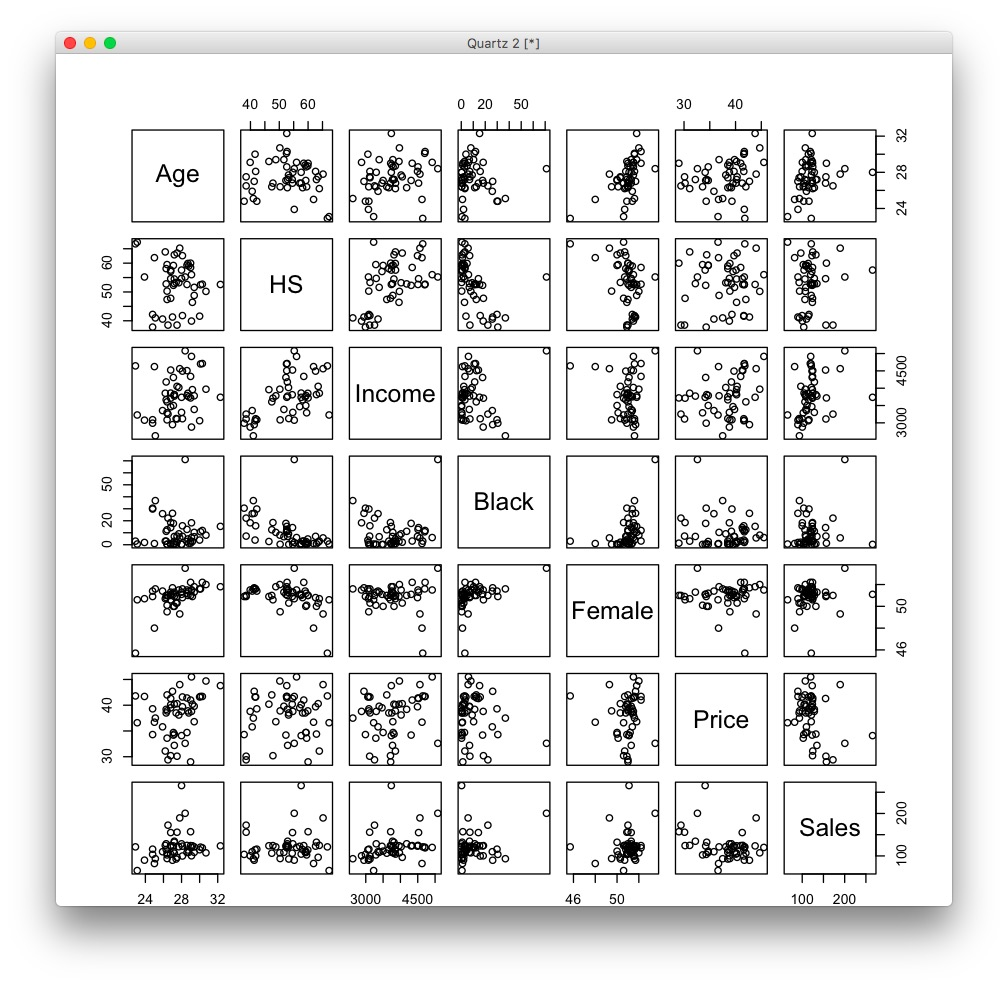
\includegraphics[width=\textwidth]{HW4.jpg}}
\end{center}



\begin{addmargin}[-1.1em]{0em}
\textbf{(c)}\par\end{addmargin}
  \textbf{Show that the three inequalities above are incompatible, using the requirements $p \in [0,1]$ and $q \in [0,1]$. What does this tell you about whether $M_2$ is in the set of rationalizable strategies?}\par
  %by putting the "\par" into the \textbf, error msg will occur...
\bigbreak
\begin{addmargin}[-0.5em]{0em}
\textbf{Answer: }\end{addmargin}


\textbf{(d)}\par\end{addmargin}
  \textbf{Argue that no pure strategy is strictly dominated in this game.}\par
  %by putting the "\par" into the \textbf, error msg will occur...
\bigbreak
\begin{addmargin}[-0.5em]{0em}
\textbf{Answer: }\end{addmargin}


\begin{addmargin}[-1.1em]{0em}
\textbf{(e)}\par\end{addmargin}
  \textbf{Combining parts (c) and (d), what has this example proved?}\par
  %by putting the "\par" into the \textbf, error msg will occur...
\bigbreak
\begin{addmargin}[-0.5em]{0em}
\textbf{Answer: }\end{addmargin}


\begin{lstlisting}
> results = lm(Sales ~ Age+HS+Income+Black+Female+Price , data=data)
> lev = hat(model.matrix(results))
\end{lstlisting}

\begin{lstlisting}
  0.148834504030601 0.580160351053579 0.0496985364502016 0.13709423363853 0.0601062187168606 0.130138939805311 0.174671432351856 0.109964259157845 0.719712840922186 0.2984807799694 0.0992462576906176 0.216903455841289 0.092060813754798 0.078138923121058 0.0863031077553889 0.0600834204236368 0.0600531614367214 0.229271714316211 0.147216983914844 0.0592277100717082 0.082438148474407 0.111768500306865 0.0788600537461464 0.0595424855799236 0.220268293959589 0.0538126742130819 0.07535749988127 0.0713061951148198 0.171156408722539 0.0663450574293963 0.112543589203342 0.205163482615724 0.125210794051503 0.189612219012305 0.0977942068782977 0.0427023659576899 0.0747312407280888 0.194824611487451 0.110848283936785 0.107728709447137 0.157387827636549 0.0702636797470909 0.0861059621640753 0.073209300335295 0.310573704010913 0.0646432821046025 0.121378178796484 0.06441386857486 0.139413729014416 0.0386706972156815 0.0845573052310269
\end{lstlisting}





%%%%%%%%%%%%%%%%%%%%%%%%%%%%%%%%%%%%%
%%%%%%%%%%%%%%   2   %%%%%%%%%%%%%%%%
%%%%%%%%%%%%%%%%%%%%%%%%%%%%%%%%%%%%%


\begin{addmargin}[-2em]{0em} \large{\textbf{2. }}\end{addmargin}
  \begin{addmargin}[-1.1em]{0em} \textbf{(a) Write down the (mathematical) definition of a pure strategy Nash equilibrium.}\par\end{addmargin}
    \textbf{}\par
  \bigbreak
  \begin{addmargin}[-0.5em]{0em}
  \textbf{Answer: }\end{addmargin}

\begin{addmargin}[-1.1em]{0em}
\textbf{(b)}\par\end{addmargin}
  \textbf{Is every strategy that is part of a pure strategy Nash equilibrium rationalizable?
}\par
   \textbf{}\par
 \bigbreak
 \begin{addmargin}[-0.5em]{0em}
 \textbf{Answer: }\end{addmargin}



\begin{addmargin}[-1.1em]{0em}
\textbf{(c)}\par\end{addmargin}
 \textbf{Write down a 2 player game in matrix form in which each player has three pure strategies, only two of which are rationalizable, and there is a unique pure strategy Nash equilibrium.
}\par

\bigbreak
\begin{addmargin}[-0.5em]{0em}
\textbf{Answer: }\end{addmargin}


%%%%%%%%%%%%%%%%%%%%%%%%%%%%%%%%%%%%%
%%%%%%%%%%%%%%   3   %%%%%%%%%%%%%%%%
%%%%%%%%%%%%%%%%%%%%%%%%%%%%%%%%%%%%%

\begin{addmargin}[-2em]{0em} \large{\textbf{3. }}\end{addmargin}

\textbf{Players 1 and 2 are bargaining over \$10. Each player $i$ names an amount, $s_i$, between 0 and 10 for herself. These numbers do not have to be in whole dollar units. The choices are made simultaneously. Each player’s payoff is equal to her own monetary payoff . We will consider this game under two different rules. In both cases, if $s_1 + s_2 \leq 10$ then the players get the amounts that they named (and the remainder, if any, is destroyed).}



\begin{addmargin}[-1.1em]{0em} \textbf{(a)}\par\end{addmargin}

\textbf{In the first case, if $s_1 +s_2 > 10$ then both players get 0 and the money is destroyed. What are all the pure strategy Nash Equilibria of this game?}\par
\bigbreak
\begin{addmargin}[-0.5em]{0em}
\textbf{Answer: }\end{addmargin}


\begin{addmargin}[-1.1em]{0em}
\textbf{(b)}\par\end{addmargin}
\textbf{In the second case, if $s_1 + s_2 > 10$ and the amounts named are different, then the person who names the smaller amount gets that amount and the other person gets the remaining money (out of 10). If $s_1 + s_2 > 10$ and $s_1 = s_2$, then both players get 5. What are all the pure strategy Nash Equilibria of this game?
}\par

\bigbreak
\begin{addmargin}[-0.5em]{0em}
\textbf{Answer: }\end{addmargin}


\begin{addmargin}[-1.1em]{0em}
\textbf{(c)}\par\end{addmargin}

\textbf{Now suppose these two games are played with the extra rule that the named amounts have to be in whole dollar units. Does this change the set of pure strategy Nash Equilibria in either case?
}\par
\bigbreak
\begin{addmargin}[-0.5em]{0em}
\textbf{Answer: }\end{addmargin}



%%%%%%%%%%%%%%%%%%%%%%%%%%%%%%%%%%%%%
%%%%%%%%%%%%%%   4   %%%%%%%%%%%%%%%%
%%%%%%%%%%%%%%%%%%%%%%%%%%%%%%%%%%%%%


\begin{addmargin}[-2em]{0em} \large{\textbf{4. }}\end{addmargin}
\textbf{Consider the following two-player game}




\begin{addmargin}[-1.1em]{0em}
\textbf{(a)}\par\end{addmargin}
\textbf{Find all pure strategy Nash Equilibria.}
\bigbreak
\begin{addmargin}[-0.5em]{0em}
\textbf{Answer: }\end{addmargin}


\begin{addmargin}[-1.1em]{0em}
\textbf{(b)}\par\end{addmargin}
\textbf{Are there other Nash equilibria, i.e. mixed strategy equilibria? If yes, list them.
}\par
\bigbreak
\begin{addmargin}[-0.5em]{0em}
\textbf{Answer: }\end{addmargin}


\bigbreak
%%%%%%%%%%%%%%%%%%%%%%%%%%%%%%%%%%%%%
%%%%%%%%%%%%%%   5   %%%%%%%%%%%%%%%%
%%%%%%%%%%%%%%%%%%%%%%%%%%%%%%%%%%%%%

\begin{addmargin}[-2em]{0em} \large{\textbf{5. }}\end{addmargin}

\textbf{A crime is observed by a group of $n > 1$ people. Each person would like the police to be informed but prefers that someone else make the phone call. Specifically, suppose that each person attaches the value $v$ to the police being informed by someone and bears a personal cost $c$ if she makes the phone call. Assume $v > c > 0$.
}

\begin{addmargin}[-1.1em]{0em}
\textbf{(a)}\par\end{addmargin}
  \textbf{Set this situation up as a simultaneous-move game: for each player, define the strategy space and the payoff function as a function of all players’ strategies.
}\par
        \bigbreak
        \begin{addmargin}[-0.5em]{0em}
        \textbf{Answer: }\end{addmargin}



\begin{addmargin}[-1.1em]{0em}
\textbf{(b)}\par\end{addmargin}
        \textbf{Is there a symmetric pure strategy Nash Equilibrium, i.e., one in which all players use the same strategy? How about asymmetric pure strategy Nash equilibria (i.e., ones in which different players can use different pure strategies)?}\par
       \bigbreak
       \begin{addmargin}[-0.5em]{0em}
       \textbf{Answer: }\end{addmargin}



\begin{addmargin}[-1.1em]{0em}
\textbf{(c)}\par\end{addmargin}
\textbf{Find a symmetric mixed strategy Nash equilibrium, i.e. one in which each person calls with the same probability. This can be done in a few steps:}\par
\bigbreak
\textbf{1. Let $p$ be the probability that each person calls in a mixed strategy equilibrium. From player $i$\’s perspective, what\’s the probability that no one else calls? What’s the probability that at least one other person calls?}\par
\bigbreak
\textbf{2. In a symmetric mixed strategy equilibrium, what must be true about a player’s expected payoff from calling and keeping silent? Write this down mathematically using the two probabilities derived in part 5(c)1.}
\bigbreak
\textbf{3. Based on the condition you derived in part 5(c)2, express p as a function of $c$ and $v$.}\par
\bigbreak
\textbf{4. In the symmetric mixed strategy equilibrium, how does p change as the size of the group increases? What about the probability that at least one person calls? What about the expected payoff of each person? Explain intuitively why the probability that crime is reported (by at least one person) increases/decreases with group size; do the same for the expected payoff of each group member.}


\begin{addmargin}[-0.5em]{0em}
\textbf{Answer: }\end{addmargin}


\end{document}


%%%%%%%%%%%%%%%%%%%%%%%%%%%%%%%%%%%%%
%%%%%%%%%%%%%%   #   %%%%%%%%%%%%%%%%
%%%%%%%%%%%%%%%%%%%%%%%%%%%%%%%%%%%%%


%Insert pics:
%%%%%%%%%%%%%
%\begin{center}
  %\makebox[\linewidth]{\includegraphics[width=\textwidth]{4640HW6.jpg}}
%\end{center}

%insert a complicated tab...
%%%%%%%%%%%%%%%%%%%%%%%%%%%%
%\begin{center}
%\begin{tabular}{ p{12cm}p{1cm}p{1cm}p{1cm}  }
%& \multicolumn{3}{c}{Posterior Quantiles} \\
%\centering{Quantity of Interest} & 25\% & 50\% & 75\% \\
%\hline
%geometric mean for Blue Earth (no basement), exp($\beta_2)$ &4.1& 5.0& 6.5\\
%geometric mean for Blue Earth County (basement), exp($\beta_1+\beta_2)$ &6.1 &7.1 &8.2\\
%geometric mean for Clay County (no basement), exp($\beta_3)$& 3.8& 4.7 &5.8\\
%geometric mean for Clay County (basement), exp($\beta_1+\beta_3)$ &5.6& 6.5& 7.6\\
%geometric mean for Goodhue County (no basement), exp($\beta_4)$ & 3.9 &4.9& 6.2\\
%geometric mean for Goodhue County (basement), exp($\beta_1+\beta_4)$ &5.8& 6.8& 7.9\\
%factor for basement vs. no basement, exp($\beta_1$)&1.1& 1.4 &1.7\\
%geometric sd of predictions, exp($\sigma$)&2.1 &2.2& 2.4\\
%\end{tabular}
%\end{center}

%%%insert code snippets:
%%%%%%%%%%%%%%%%%%%%%%%%
%\begin{lstlisting}
%INSERT CODE HERE
%\end{lstlisting}

%%insert equation with severl lines:
%\begin{align}
%LEFT &= RIGHT1 \nonumber\\
%     &= RIGHT2 \nonumber\\
%     &= RIGHT3 \nonumber
%\end{align}


%ssh-add ~/.ssh/id_rsa
